\newpage
\section{Auswertung}
\noindent
Die aufgenommenen Messdaten zur Untersuchung des Selektivverstärkers sind in Tabelle (\ref{tab:selektiv}) aufgeführt.
Dabei wurde die Ausgangsspannung $U_A$ in Abhängigkeit von der Frequenz $\nu$ bei konstanter Eingangsspannung $U_E$ = 495 mV und der Güte Q = 100 gemessen.
Die dazugehörige Filterkurve ist in Abbildung (\ref{fig:selektiv}) dargestellt, 
wo bei einer Frequenz von 35.5 kHz ein Maximum von $U_A =$ 5.36 V
zu beobachten ist.

\begin{figure}
    \centering
       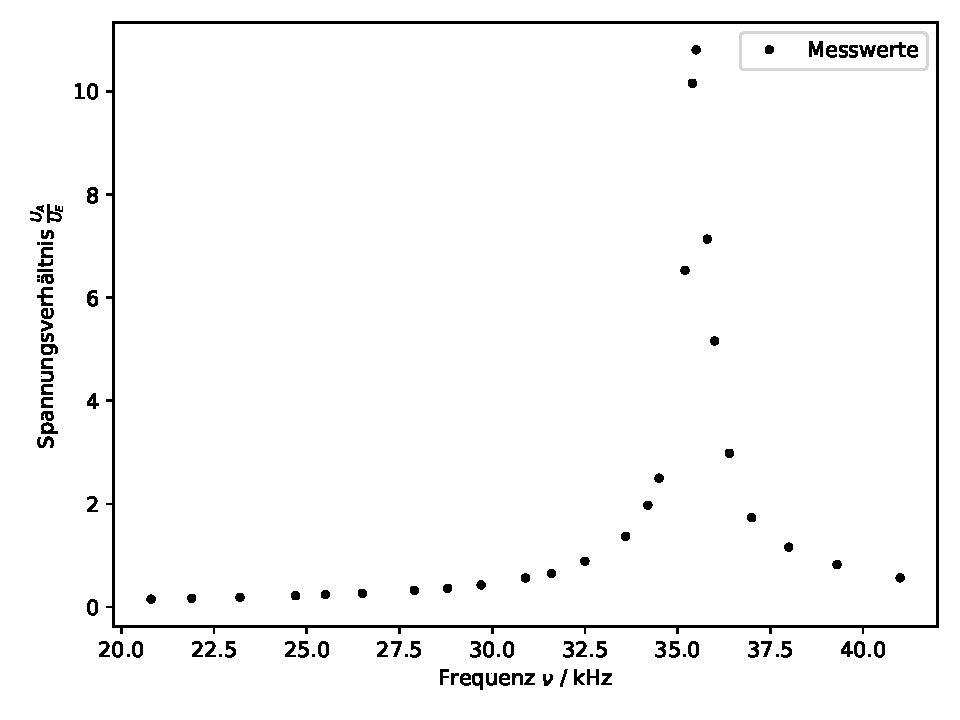
\includegraphics[width=\textwidth]{selektiv.pdf}
       \caption{Filterkurve des Selektivverstärkers.}
       \label{fig:selektiv}
\end{figure}

\begin{table}
\centering
\begin{tabular}{c c}
\toprule
{$\nu \mathbin{/} \si{\kilo\hertz} $} & {$U_A \mathbin{/} \si{\milli\volt}$}  \\
\midrule
20.8  &    76 \\
21.9  &    84 \\
23.2  &    94 \\
24.7  &   108 \\
25.5  &   120 \\
26.5  &   132 \\
27.9  &   160 \\
28.8  &   180 \\
29.7  &   212 \\
30.9  &   280 \\
31.6  &   324 \\
32.5  &   440 \\
33.6  &   680 \\
34.2  &   980 \\
34.5  &  1240 \\
35.2  &  3240 \\
35.4  &  5040 \\
35.5  &  5360 \\
35.8  &  3540 \\
36    &  2560 \\
36.4  &  1480 \\
37    &   860 \\
38    &   576 \\
39.3  &   408 \\
41    &   280 \\
\bottomrule
\end{tabular}
\caption{Messdaten zur Untersuchung der Filterkurve.}
\label{tab:selektiv}
\end{table}

\newpage
\noindent
Für die experimentelle Bestimmung der Suszeptibilitäten werden zunächst die Daten der beiden Proben aufgenommen.
In Tabelle (\ref{tab:proben}) sind die Masse $m$, die Dichte $\rho$ und die Länge $l$, 
die sich aus der tatsächlich eingeführten Länge ohne Löcher zusammensetzt, aufgeführt.
Außerdem befindet sich dort der reale Querschnitt $Q_{real}$ 
der aus den aufgeführten Daten nach 

\begin{equation}
Q_real = \frac{m}{l\rho}
\end{equation}

\noindent
berechnet wird.

\begin{table}
    \centering
    \begin{tabular}{c c c c c}
        \toprule
        {Stoff} & {$m \mathbin{/} \si{\gram}$} & {$\rho \mathbin{/} \si[per-mode=fraction]{\gram\per\cubic\centi\meter}$} & {$l \mathbin{/} \si{\centi\meter}$} & {$Q_{real} \mathbin{/} \si{\centi\meter\squared}$} \\
    \midrule
    $\ce{Dy2O3}$ & 15.1  & 7.8 & 14.8 & 0.131 \\
    $\ce{Gd2O3}$ & 14.08 & 7.4 & 15.5 & 0.123 \\
    \bottomrule
\end{tabular}
\caption{Daten der Proben.}
\label{tab:proben}
\end{table}

\noindent
In Tabelle (\ref{tab:exp1}) und (\ref{tab:exp2}) befinden sich die gemessenen die Brückenspannungen $U_o$ ohne Probe nach Abgleich und $U_m$ mit Probe sowie die dazugehörigen Widerstände
$R_o$ ohne Probe und $R_m$ mit Probe und Differenzen. 

\begin{table}
    \centering
    \begin{tabular}{c c c c c c}
        \toprule
        {$U_o \mathbin{/} \si{\milli\volt}$} & {$U_m \mathbin{/} \si{\milli\volt}$} & {$R_o \mathbin{/} \si{\ohm}$} & {$R_m \mathbin{/} \si{\ohm}$} & {$\Delta U \mathbin{/} \si{\milli\volt}$} & {$\Delta R \mathbin{/} \si{\ohm}$} \\
    \midrule
    0.5     &   3.8   &     3.215     &     1.645    &   3.3   &  1.57  \\
    0.55    &   3.79  &     3.210     &     1.65     &   3.24  &  1.56  \\ 
    0.52    &   3.7   &     3.175     &     1.597    &   3.18  &  1.579 \\
    \bottomrule
\end{tabular}
\caption{Messdaten und Differenzen von $\ce{Dy2O3}$.}
\label{tab:exp1}
\end{table}

\begin{table}
    \centering
    \begin{tabular}{c c c c c c}
        \toprule
        {$U_o \mathbin{/} \si{\milli\volt}$} & {$U_m \mathbin{/} \si{\milli\volt}$} & {$R_o \mathbin{/} \si{\ohm}$} & {$R_m \mathbin{/} \si{\ohm}$} & {$\Delta U \mathbin{/} \si{\milli\volt}$} & {$\Delta R \mathbin{/} \si{\ohm}$} \\
    \midrule
    0.51    &   1.19   &     3.223     &     2.437    &   1.4   &  0.786  \\
    0.5     &   1.79   &     3.144     &     2.422    &   1.29  &  0.722  \\ 
    0.5     &   1.95   &     3.222     &     2.422    &   1.45  &  0.8    \\
    \bottomrule
\end{tabular}
\caption{Messdaten und Differenzen von $\ce{Gd2O3}$.}
\label{tab:exp2}
\end{table}

\noindent 
Die Spule in die die Proben eingeführt werden hat einen Querschnitt von $F=0.866\si{\centi\meter\squared}$ und $N=250$ Wicklungen.
Damit lassen sich die Suszeptibilitäten $\chi_U$ nach Formel (\ref{eqn:spannung})
und $\chi_R$ nach Formel (\ref{eqn:alternativ})
bestimmen.
Die experimentell bestimmten Suszeptibilitäten befinden sich in Tabelle (\ref{tab:expsus}).

\begin{table}
    \centering
    \begin{tabular}{c c c}
        \toprule
        {Stoff} & {$\chi_U $} & {$\chi_R $} \\
    \midrule
    $\ce{Dy2O3}$ & 0.1730 $\pm$ 0.0026  &  0.0208 $\pm$ 0.0001 \\
    $\ce{Gd2O3}$ & 0.0785 $\pm$ 0.0038  & 0.0109  $\pm$ 0.0005 \\
    \bottomrule
\end{tabular}
\caption{Mittelwert und Standardabweichung der experimentell bestimmten Suszeptibilitäten.}
\label{tab:expsus}
\end{table}

\newpage
\noindent
Nun werden die theoretischen Suszeptibilitäten bestimmt.
Dazu werden einige atomare Daten der Stoffe wie die Quantenzahlen und die molare Masse M in Tabelle (\ref{tab:th1}) gesammelt, aus denen sich der Landé-Faktor $g_J$ nach Formel (\ref{eqn:lande})
berechnen lässt.
Mit den gesammelten Daten lassen sich die theoretischen Suszeptibilitäten $\chi_T$ nach Formel (\ref{eqn:theo}) mit T=293.15 K und $N$ nach 

\begin{equation}
N = \frac{2\rho N_A}{M}
\end{equation}

\noindent
bestimmen. 
Dabei ist $N_A$ die Avogadrokonstante.


\begin{table}
    \centering
    \begin{tabular}{c c c c c c c c}
        \toprule
        {Stoff} & {L} & {S} & {J} & {M $\mathbin{/} \si[per-mode=fraction]{\gram\per\mol}$ } & {$g_J$} & {N $\cdot 10^{28} \mathbin{/} \si[per-mode=fraction]{\per\cubic\meter} $} & {$\chi_T$} \\
    \midrule
    $\ce{Dy2O3}$ & 5 & 2.5 & 7.5 & 372.998 & 1.33 & 2.519 & 0.0254 \\
    $\ce{Gd2O3}$ & 0 & 3.5 & 3.5 & 362.49  & 2    & 2.649 & 0.0149 \\
    \bottomrule
\end{tabular}
\caption{Atomare Daten der Stoffe und theoretische Suszeptibilitäten.}
\label{tab:th1}
\end{table}